\documentclass[10pt,letterpaper]{article}
\usepackage[utf8]{inputenc}
\usepackage[T1]{fontenc}
\usepackage[margin=0.6in]{geometry}
\usepackage{amsmath,amssymb,mathtools,graphicx,booktabs,xcolor,hyperref}
\setlength{\parindent}{0pt}
\setlength{\parskip}{5pt}
\begin{document}

\section*{Block S5 Exercises: Series AC RLC Concepts, Inductance, Reactance \& Capacitance}

  \textbf{Schedule Window:} Sunday, Oct 18, 8:00--9:00 PM (60 min) ~|~
  \textbf{Total Points:} 44 pts ~|~
  \textbf{Mix:} 2 Calculus Derivations, 1 10-Blank Cloze, 1 Spec v2 AC RLC FR, 2 Graphs + Phasors



  \textbf{Core Mastery Goals:} (1) Deriving $X_L = \omega L$ ($+90^\circ$ voltage lead) and $X_C = \frac{1}{\omega C}$ ($-90^\circ$ voltage lag) from $v_L = L\frac{di}{dt}$ and $i_C = C\frac{dv_C}{dt}$; (2) Deriving solenoid inductance $L = \frac{\mu_0 N^2 A}{\ell}$ and magnetic energy density $u_B = \frac{B^2}{2\mu_0}$; (3) Mastering series impedance $Z = \sqrt{R^2 + (X_L - X_C)^2}$, phase angle $\phi$, and series resonance $\omega_0 = \frac{1}{\sqrt{LC}}$.


\subsection*{01 $\cdot$ Calculus Proofs: Inductive/Capacitive Reactance \& Solenoid Energy Density \hfill [Ch. 30--31 $\cdot$ 12 Points $\cdot$ DERIVE]}

\begin{enumerate}
  \item \textbf{Inductive Reactance $X_L = \omega L$ \& Capacitive Reactance $X_C = \frac{1}{\omega C}$ [6 points]:} Suppose a steady sinusoidal AC current $i(t) = I_0 \cos(\omega t)$ with angular frequency $\omega$ (in $\text{rad/s}$) and amplitude $I_0$ flows through a series circuit.
    \begin{enumerate}
      \item Substitute $i(t) = I_0\cos(\omega t)$ into Faraday's inductor relation $v_L(t) = L\dfrac{di}{dt}$, use the trigonometric identity $-\sin(\omega t) = \cos(\omega t + \frac{\pi}{2})$, and prove that the peak inductor voltage is $V_{L,0} = I_0 X_L$ where $X_L = \omega L$, with $v_L(t)$ \textbf{leading} $i(t)$ by $+90^\circ$ ($+\frac{\pi}{2}\text{ rad}$). \textbf{[3 pts]}
      \item Integrate $v_C(t) = \dfrac{1}{C}\int i(t)\,dt$ (with zero DC offset) or differentiate $i(t) = C\dfrac{dv_C}{dt}$, use $\sin(\omega t) = \cos(\omega t - \frac{\pi}{2})$, and prove that the peak capacitor voltage is $V_{C,0} = I_0 X_C$ where $X_C = \dfrac{1}{\omega C}$, with $v_C(t)$ \textbf{lagging} $i(t)$ by $-90^\circ$ ($-\frac{\pi}{2}\text{ rad}$). \textbf{[3 pts]}
    \end{enumerate}
  
  \item \textbf{Solenoid Self-Inductance \& Magnetic Field Energy Density [6 points]:} Consider a long, tightly wound ideal solenoid of length $\ell$, cross-sectional area $A$, and $N$ total turns carrying current $I$, as shown below.
  \begin{center}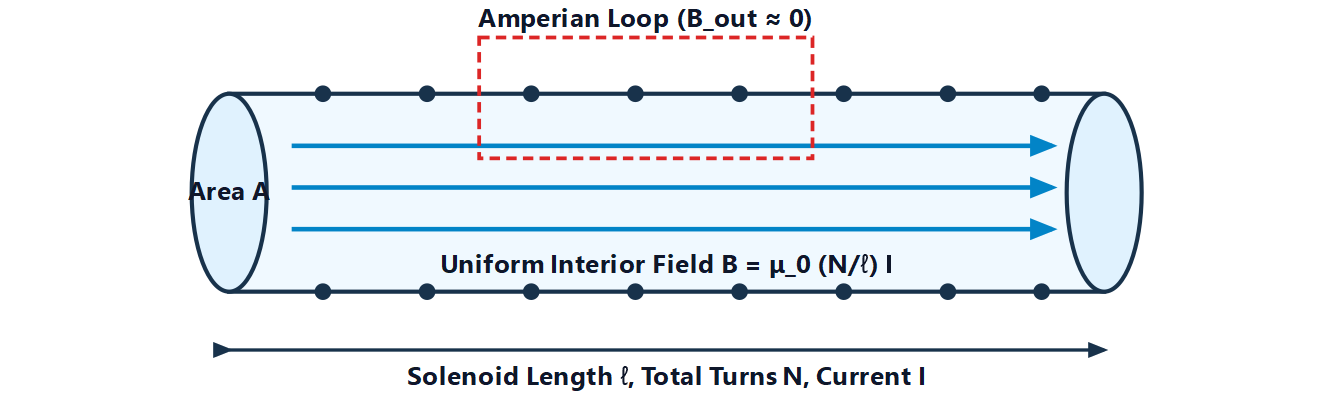
\includegraphics[width=0.82\linewidth]{day1_assets/s5-q1-solenoid.png}\end{center}
    \begin{enumerate}
      \item Apply Amp\`ere's law $\oint \mathbf{B}\cdot d\mathbf{l} = \mu_0 I_{\text{enc}}$ around the dashed rectangular Amperian loop to find the uniform interior magnetic field $B$, compute the total flux linkage $N\Phi_B = N(BA)$, and prove from $N\Phi_B = LI$ that the solenoid's self-inductance is:
      $$L = \frac{\mu_0 N^2 A}{\ell}.$$ \textbf{[3 pts]}
      \item Integrate the instantaneous magnetic power $dU_B = v_L i\,dt = L i\,di$ from $i' = 0$ to $i' = I$ to prove $U_B = \frac{1}{2}LI^2$, and divide by the interior volume $V_{\text{vol}} = A\ell$ to prove that the magnetic energy density stored in any magnetic field $B$ in vacuum is:
      $$u_B = \frac{U_B}{A\ell} = \frac{B^2}{2\mu_0}.$$ \textbf{[3 pts]}
    \end{enumerate}
  
\end{enumerate}
\vspace{1.2in}


\newpage



\subsection*{02 $\cdot$ Conceptual Cloze: Inductance, Reactance, Phase \& Series AC RLC Resonance \hfill [Ch. 30--31 $\cdot$ 10 Points $\cdot$ CLOZE]}

Complete each statement below using the exact term or expression from the 14-item word bank (each item used at most once; four items are unused distractors).


  \textbf{WORD BANK:} ~
  \texttt{electric field} $\cdot$
  \texttt{magnetic field} $\cdot$
  \texttt{leads} $\cdot$
  \texttt{lags} $\cdot$
  \texttt{in phase with} $\cdot$
  \texttt{short circuit ($X_L \to 0$)} $\cdot$
  \texttt{open circuit ($X_C \to \infty$)} $\cdot$
  \texttt{$\sqrt{R^2 + (X_L - X_C)^2}$} $\cdot$
  \texttt{$R + X_L - X_C$} $\cdot$
  \texttt{$1/\sqrt{LC}$} $\cdot$
  \texttt{minimum ($Z = R$)} $\cdot$
  \texttt{maximum ($Z \to \infty$)} $\cdot$
  \texttt{capacitive ($\phi < 0$)} $\cdot$
  \texttt{$\cos\phi = R/Z$}


\begin{enumerate}
  \item \textbf{[1 pt]} Whereas a charged capacitor stores potential energy $U_C = \frac{1}{2}CV^2 = \frac{1}{2}\varepsilon_0 E^2 (Ad)$ in its electric field, a current-carrying inductor stores potential energy $U_L = \frac{1}{2}LI^2 = \frac{B^2}{2\mu_0}(A\ell)$ in its \underline{\hspace{1.8in}}.
  \item \textbf{[1 pt]} Across an ideal resistor $R$, the instantaneous AC voltage $v_R(t)$ is always \underline{\hspace{1.8in}} the current $i(t)$ ($\phi_R = 0^\circ$).
  \item \textbf{[1 pt]} Across an ideal inductor $L$, the terminal voltage $v_L(t) = L\frac{di}{dt}$ \underline{\hspace{1.8in}} the current $i(t)$ by $90^\circ$ (mnemonic: \textbf{ELI}).
  \item \textbf{[1 pt]} Across an ideal capacitor $C$, the terminal voltage $v_C(t) = \frac{1}{C}\int i\,dt$ \underline{\hspace{1.8in}} the current $i(t)$ by $90^\circ$ (mnemonic: \textbf{ICE}).
  \item \textbf{[1 pt]} In the low-frequency DC limit ($\omega \to 0$), an ideal inductor has $X_L \to 0$ (a short circuit), whereas an ideal capacitor acts as an \underline{\hspace{1.8in}}.
  \item \textbf{[1 pt]} Because $\vec{V}_R$ is perpendicular to $(\vec{V}_L + \vec{V}_C)$ on the phasor diagram, the total impedance of a series RLC circuit is the Pythagorean sum $Z =$ \underline{\hspace{1.8in}} rather than an algebraic sum.
  \item \textbf{[1 pt]} Series resonance occurs when $X_L(\omega_0) = X_C(\omega_0)$, which yields the resonant angular frequency $\omega_0 =$ \underline{\hspace{1.8in}}.
  \item \textbf{[1 pt]} At series resonance ($\omega = \omega_0$), the inductive and capacitive voltage phasors cancel ($V_L = V_C$), so the total impedance $Z$ reaches its absolute \underline{\hspace{1.8in}} and the current amplitude $I_0 = V_0/R$ is maximized.
  \item \textbf{[1 pt]} When a series RLC circuit is driven below resonance ($\omega < \omega_0$), $X_C > X_L$ and the net circuit behavior is \underline{\hspace{1.8in}}, meaning the source voltage $v_s(t)$ lags behind the current $i(t)$.
  \item \textbf{[1 pt]} Ideal inductors and capacitors absorb zero net energy over a full cycle; the time-averaged power delivered by the AC source is $P_{\text{avg}} = V_{\text{rms}} I_{\text{rms}} \cos\phi = I_{\text{rms}}^2 R$, where the quantity \underline{\hspace{1.8in}} is called the \textbf{power factor}.
\end{enumerate}


  \textbf{Quick Self-Check Question (write 2 sentences below):} Why can the peak voltage $V_{C,0} = I_0 X_C$ across the capacitor in a series RLC circuit at resonance exceed the peak source voltage $V_0$ (whenever $X_C(\omega_0) > R$) without violating Kirchhoff's loop rule?

\vspace{1.2in}


\newpage



\subsection*{03 $\cdot$ Series AC RLC Circuit Analysis Across Three Driving Frequencies \hfill [Ch. 31 $\cdot$ 12 Points $\cdot$ FR + SPEC V2]}

In the Spec v2 series AC RLC circuit below, a sinusoidal voltage source $v_s(t) = V_0 \cos(\omega t)$ with fixed peak amplitude $V_0 = 120\text{ V}$ drives a series combination of $R = 50.0\ \Omega$, $L = 0.200\text{ H}$, and $C = 20.0\ \mu\text{F}$.

\begin{center}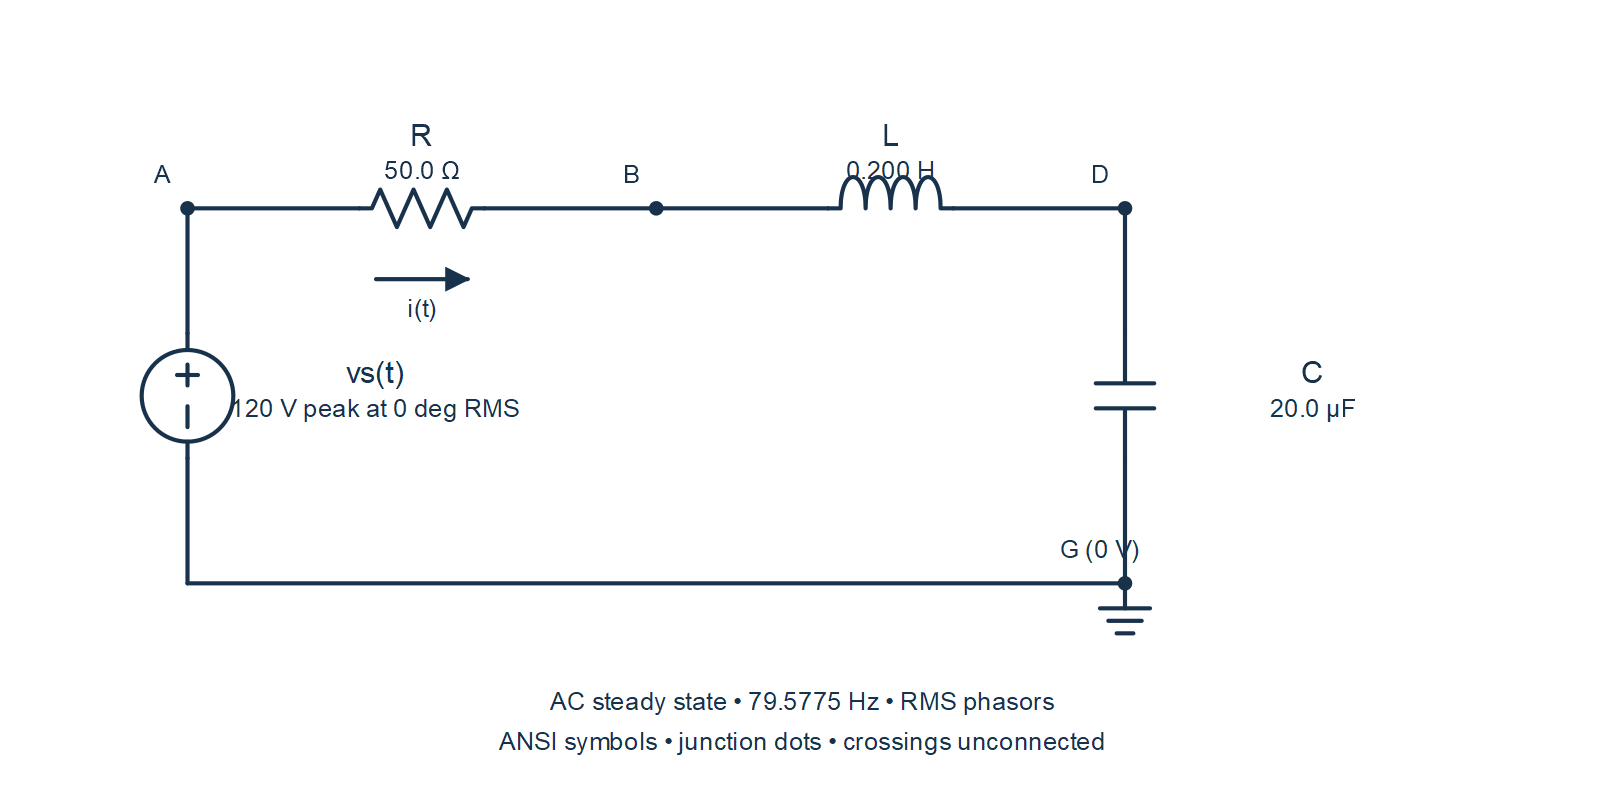
\includegraphics[width=0.82\linewidth]{day1_assets/s5-q3-ac-rlc.png}\end{center}

\begin{enumerate}
  \item \textbf{Resonant Frequency \& Resonance State ($\omega = \omega_0$) [4 points]:}
    \begin{enumerate}
      \item Calculate the resonant angular frequency $\omega_0 = \dfrac{1}{\sqrt{LC}}$ (in $\text{rad/s}$) and the corresponding linear frequency $f_0 = \dfrac{\omega_0}{2\pi}$ (in $\text{Hz}$).
      \item At $\omega = \omega_0$, compute $X_L(\omega_0)$, $X_C(\omega_0)$, the total impedance $Z(\omega_0)$, the peak current $I_0(\omega_0)$, the phase angle $\phi$, the time-averaged power $P_{\text{avg}} = \frac{1}{2}I_0^2 R$, and the peak voltages $V_{R,0}, V_{L,0}, V_{C,0}$. Explain how your values of $V_{L,0}$ and $V_{C,0}$ are consistent with KVL and $V_0 = 120\text{ V}$.
    \end{enumerate}
  
  \item \textbf{Low-Frequency Operation ($\omega_1 = 250\text{ rad/s}$) [4 points]:}
    \begin{enumerate}
      \item At $\omega_1 = 250\text{ rad/s}$, compute $X_L(\omega_1)$, $X_C(\omega_1)$, the net reactance $X(\omega_1) = X_L - X_C$, and the impedance $Z(\omega_1) = \sqrt{R^2 + (X_L - X_C)^2}$.
      \item Find the current amplitude $I_0(\omega_1)$, the phase angle $\phi_1 = \arctan\left(\dfrac{X_L - X_C}{R}\right)$ (in degrees), the power factor $\cos\phi_1$, the average power $P_{\text{avg}}(\omega_1)$, and write the steady-state current $i(t) = I_0\cos(\omega_1 t - \phi_1)$.
    \end{enumerate}
  
  \item \textbf{High-Frequency Operation ($\omega_2 = 1000\text{ rad/s}$) [4 points]:}
    \begin{enumerate}
      \item At $\omega_2 = 1000\text{ rad/s}$, compute $X_L(\omega_2)$, $X_C(\omega_2)$, $X(\omega_2) = X_L - X_C$, $Z(\omega_2)$, $I_0(\omega_2)$, $\phi_2$ (in degrees), and $P_{\text{avg}}(\omega_2)$.
      \item Compare your results at $\omega_1 = 250\text{ rad/s}$ and $\omega_2 = 1000\text{ rad/s}$: how do $Z$, $I_0$, $P_{\text{avg}}$, and the phase angle $\phi$ compare between these two frequencies, and why?
    \end{enumerate}
  
\end{enumerate}
\vspace{1.2in}


\newpage



\subsection*{04 $\cdot$ Frequency-Response Graphs \& Voltage Phasor Diagrams \hfill [Ch. 31 $\cdot$ 10 Points $\cdot$ 2 DRAW]}

For the series AC RLC circuit of Exercise 03 ($V_0 = 120\text{ V}, R = 50.0\ \Omega, L = 0.200\text{ H}, C = 20.0\ \mu\text{F}$):

\begin{enumerate}
  \item \textbf{Graph (i) --- Reactances \& Impedance vs. Angular Frequency [3 points]:} On the top-left grid below, plot $X_L(\omega) = \omega L$, $X_C(\omega) = \frac{1}{\omega C}$, and $Z(\omega) = \sqrt{R^2 + (X_L - X_C)^2}$ (\textbf{dependent variables}, vertical axis, in $\Omega$) vs. driving angular frequency $\omega$ (\textbf{independent variable}, horizontal axis, in $\text{rad/s}$) from $\omega = 0$ to $\omega = 1000\text{ rad/s}$. Label the coordinates of the reactance crossover point where $X_L(\omega_0) = X_C(\omega_0)$ and the minimum impedance point $(\omega_0, Z_{\min})$.
  \item \textbf{Graph (ii) --- Resonance Current Curve for Low $R$ vs. High $R$ [3 points]:} On the top-right grid below, plot the current amplitude $I_0(\omega) = \frac{V_0}{Z(\omega)}$ (\textbf{dependent variable}, vertical axis, in $\text{A}$) vs. driving angular frequency $\omega$ (\textbf{independent variable}, horizontal axis, in $\text{rad/s}$) for (1) $R = 50.0\ \Omega$ and (2) $R = 120\ \Omega$. Label the resonant frequency $\omega_0$ and the peak current $I_{0,\max}$ for each curve.
  \item \textbf{Diagrams (iii) \& (iv) --- Voltage Phasor Diagrams [4 points]:} On the bottom axes (where the current phasor $\vec{I}_0$ lies along the $+x$ reference axis at $0^\circ$), draw to scale the individual voltage phasors $\vec{V}_R$, $\vec{V}_L$, $\vec{V}_C$, the net reactive phasor $\vec{V}_L + \vec{V}_C$, and the resultant source phasor $\vec{V}_s = \vec{V}_R + (\vec{V}_L + \vec{V}_C)$, and label the phase angle $\phi$ and whether the circuit is capacitive or inductive for:
    \begin{itemize}
      \item \textbf{(iii) $\omega_1 = 250\text{ rad/s}$} (using your values from Exercise 03b).
      \item \textbf{(iv) $\omega_2 = 1000\text{ rad/s}$} (using your values from Exercise 03c).
    \end{itemize}
  
\end{enumerate}

\begin{center}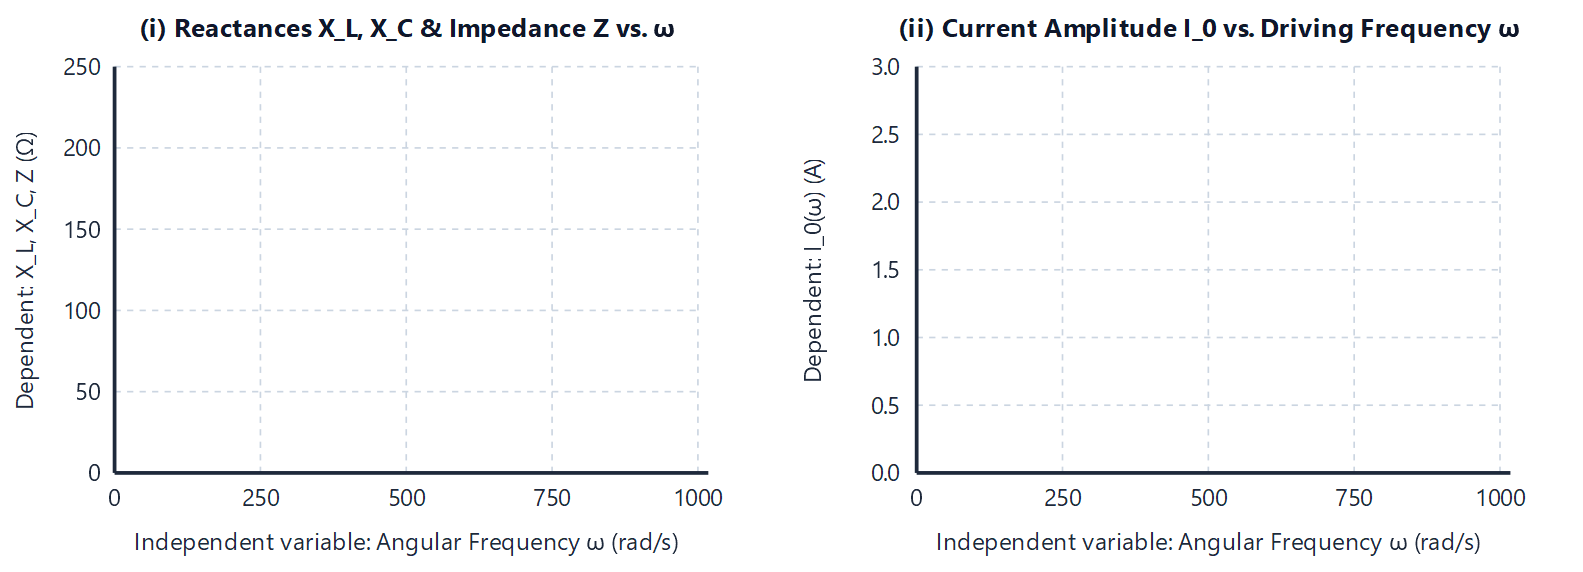
\includegraphics[width=0.82\linewidth]{day1_assets/s5-q4-grid-blank.png}\end{center}
\begin{center}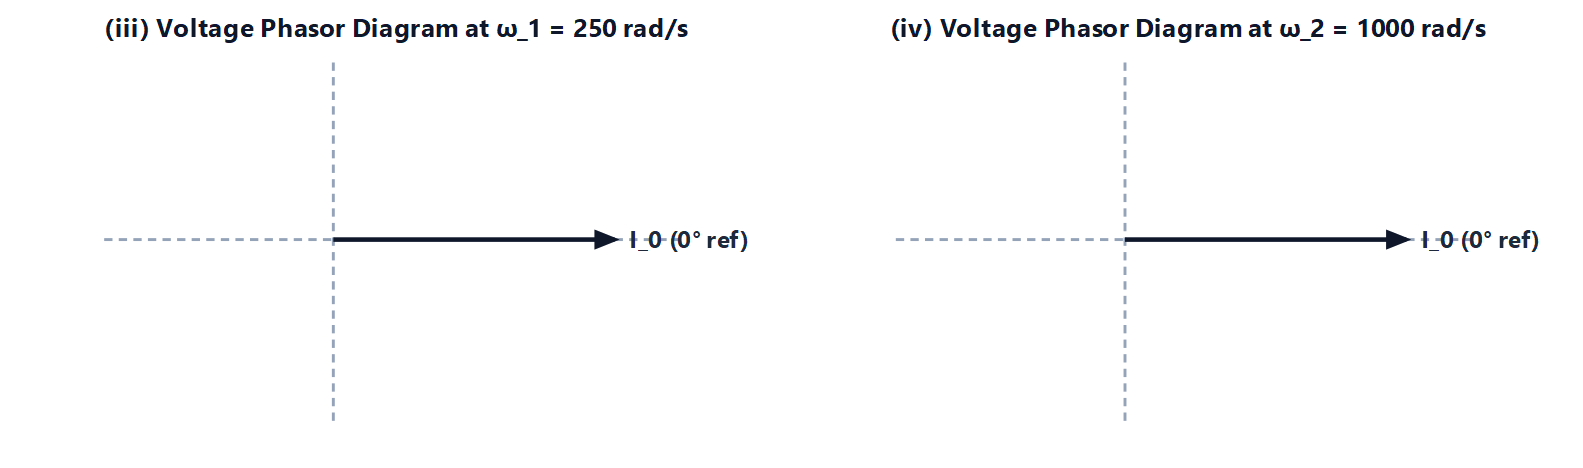
\includegraphics[width=0.82\linewidth]{day1_assets/s5-q4-phasors-blank.png}\end{center}

\end{document}
